%%%%%%%%%%%%%%%%%%%%%%%%%%%%%%%%%%%%%%%%%%%%%%%%
% BOZZA PER TESI DI LAUREA IN LATEX
%%%%%%%%%%%%%%%%%%%%%%%%%%%%%%%%%%%%%%%%%%%%%%%%

%\documentclass[12pt,titlepage]{book}
\documentclass[a4paper,twoside,12pt]{article}
\usepackage[british]{babel}
\usepackage{gensymb}
%\usepackage{graphics}
%\usepackage{url,amsfonts,epsfig}
%\usepackage[applemac]{inputenc} %comando per le lettere accentate se usate mac  
\usepackage[utf8]{inputenc} % comando per le lettere accentate se usate pc  
\usepackage[nottoc]{tocbibind}
\usepackage{unipitesi}
\usepackage{hyperref}
\usepackage{graphicx}
\usepackage{verbatim}
\graphicspath{ {Images/} }

\hypersetup{
colorlinks=true,
linkcolor=blue,
urlcolor=blue
}
\urlstyle{same}

%\title{\textsc{Analysis of performance of ATLAS experiment Phase 2 inner tracker}}
%\author{Federico Massa}

\begin{document}

%%%% Opzione per interlinea 2
%%%\baselineskip 18pt

%\maketitle

\titolo{\textit{Studio delle prestazioni dei} \\
			\textit{ layout di ITk nelle misure di $H\rightarrow ZZ^{*}\rightarrow 4\mu$ }}
\laureando{Federico Massa} 
\corsodilaureamagistrale{Fisica} 
\relatore[Prof.]{Giorgio Chiarelli} 
%\secondorelatore[Prof.]{prof2} s
%\controrelatore[Prof.]{prof3} 
\annoaccademico{2015-2016} 
\data{data}
\maketitle


\tableofcontents
%%\listoffigures
%%\listoftables
\newpage

\begin{abstract}
La fase di High Luminosity LHC offrirà nuove opportunità per esplorare eventi estremamente rari, ed in particolare per studiare la fisica e le proprietà del bosone di Higgs.
L’esperimento ATLAS, per sfruttare al massimo questa possibilità, sostituirà l’Inner Tracker  all’attuale Inner Detector.
A causa dell'elevato numero di eventi di pileup ($>200$) previsti, il tempo richiesto dalla simulazione Monte Carlo risulta proibitivo. E’ stato, pertanto, sviluppato un metodo ad-hoc che permette di simulare solo le regioni di interesse in modo accurato, confrontando differenti configurazioni del rivelatore. In questo studio presentero' i risultati ottenuti relativamente al canale\\ {$H\rightarrow ZZ^*\rightarrow 4\mu$}
\end{abstract}

\newpage

\section{Introduction} \label{Introduction}
The Large Hadron Collider (LHC) accelerator is scheduled to be upgraded in two different stages: the first one will begin after the end of Run 2 during the Long Shotdown 2 (LS2) in 2019-2020; the second one will start at the end of Run 3 during the Long Shotdown 3 (LS3) in 2024-2026 (Fig.\ref{fig:HLLHC_Plan}). The latter upgrade stage will lead to what is known as High-Luminosity LHC (HL-LHC) during which the
luminosity will reach the maximum value of $7.5 \times 10^{34}\ cm^{-2}s^{-1}$, corresponding to approximately $3000\ fb^{-1}$ during ten years of data taking. \\

\begin{figure} [h]
	\includegraphics[width=\textwidth]{HLLHC_Plan}
	\caption{LHC/HL-LHC Plan as scheduled in 2015\cite{scoping}.}
	\label{fig:HLLHC_Plan}
\end{figure}

HL-LHC will allow to study new physics processes, such as extra dimensions or the ones predicted by SUSY models, as well as improve Standard Model measurements. In particular, Higgs boson 
couplings are expected to be measured with a precision between 5\% and 30\%\cite{loi}. Thanks to the increased luminosity, it will be possible to observe the Higgs boson in rare
channels such as  $H \rightarrow \mu\mu$, vector boson 
fusion production of $H \rightarrow \gamma\gamma$ and $H \rightarrow \tau\tau$, associated production $t\bar{t}H$ with $H \rightarrow \gamma\gamma$, as well as Higgs self couplings
such as in $HH \rightarrow \tau\tau b b$, $HH \rightarrow \gamma\gamma b b$.\\

By the end of Run 3, ATLAS detector will be using 15-20 years old components. In particular,
the highly irradiated Inner Detector pixels and strips will have reached the end of their
lifetime and the transition radiation tracker will reach 100\% occupancy at that luminosity. Thus, the Inner Detector will have to be completely substituted by the Inner Tracker (ITk), which will
have to guarantee the same or an improved performance in the harsh conditions of HL-LHC while maximizing the acceptance. At the design luminosity, the expected number of in-time pileup events will be $<\mu > = 200$, a much
higher value than the one expected at the end of Run 3 ($<\mu > = 80$) and even more if 
compared to the current one ($<\mu > = 35$??), introducing new challenges in the pattern
recognition. The increase of the number
of collisions per bunch crossing leads to new requirements on the front-end electronics, trigger and data acquisition system that cannot be met by the current apparatus, thus leading to a 
substantial upgrade of the electronics. Moreover, in the Reference Scenario of the Scoping Document\cite{scoping} the geometrical acceptance of ATLAS detector is increased with respect to 
the current one thanks to the extension of the $|\eta|$ coverage to $4.0$, which requires either the substitution (such as in the case of ITk) or the addition of new detectors (muon chambers,
calorimeter system). \\

Other than detector and hardware upgrades, HL-LHC will require software upgrades to meet the needs of the upgraded detectors, handle large event samples and adapt to multi-processor
architectures. To deal with the simulation size and time requirements it will be necessary to mix fast simulation techniques (using detector parametrisations) with full simulation at event level.






\subsection{Coordinate system - perigee parameters definition - maybe in appendix}


\newpage

\section{Detector} \label{Detector}

\begin{figure} [h]
	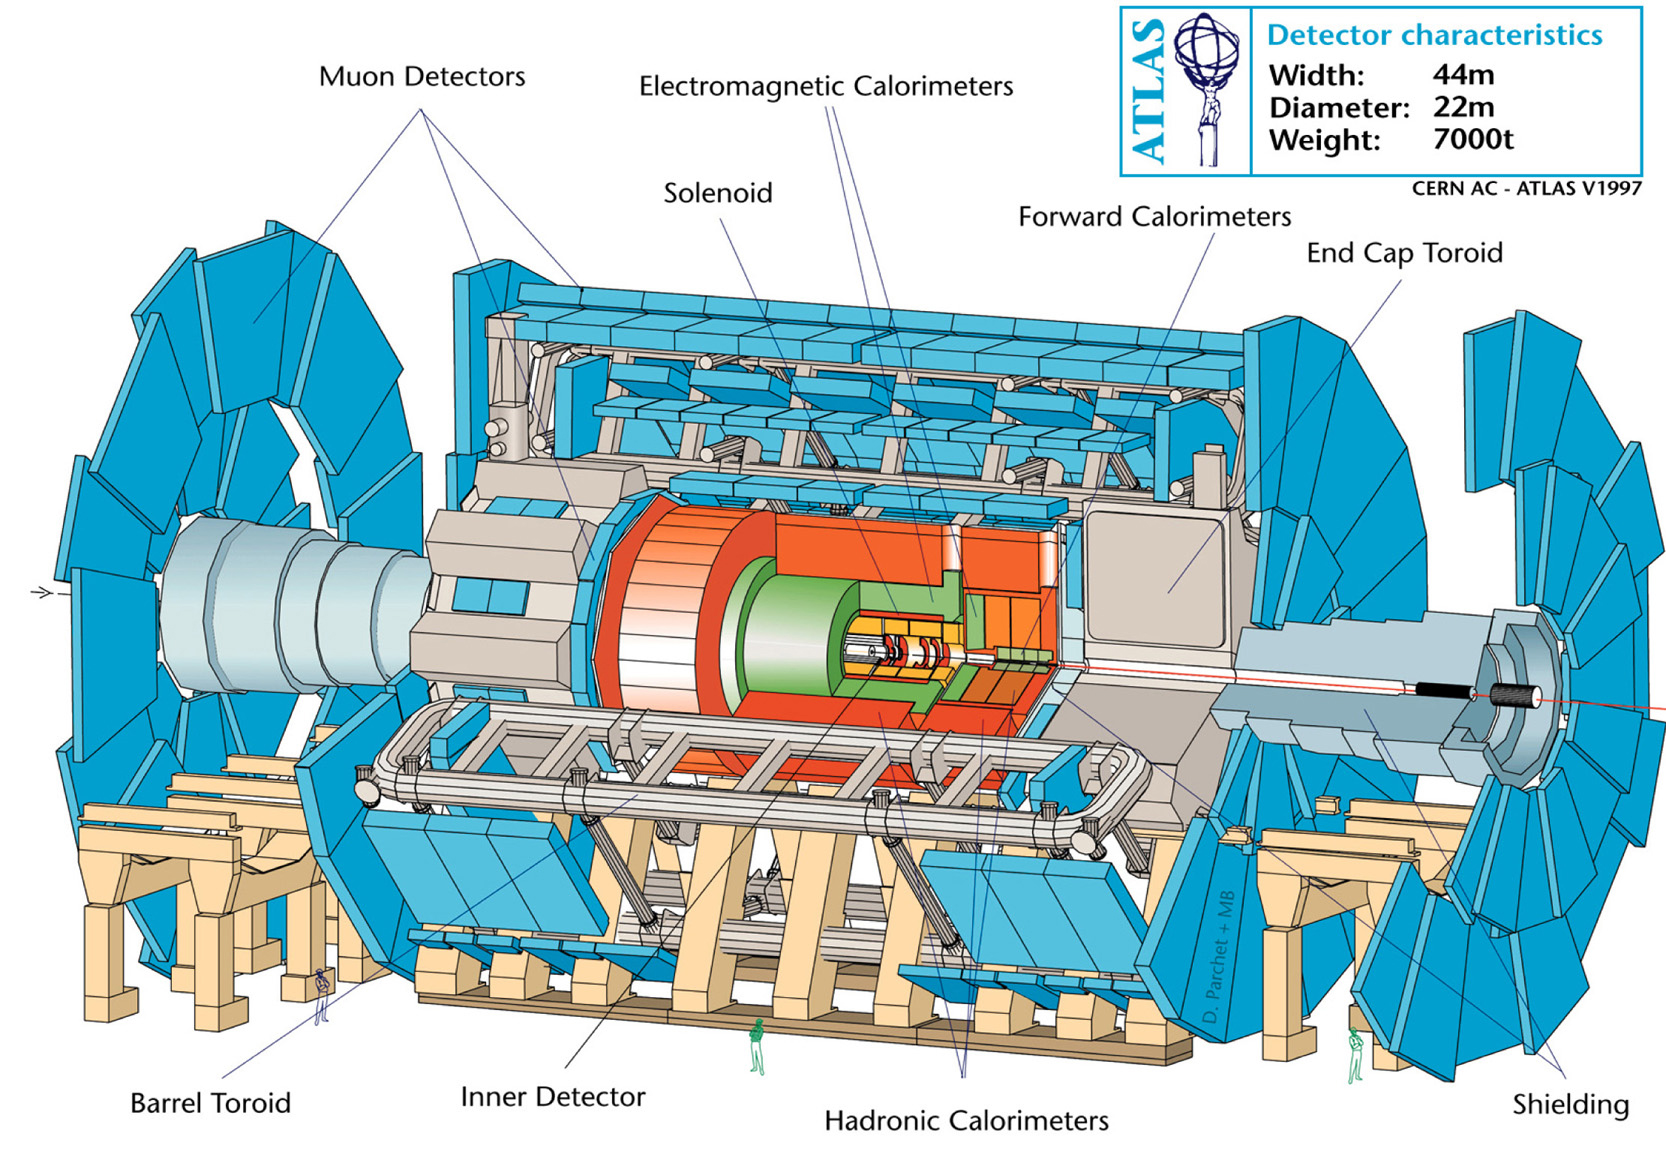
\includegraphics[width=\textwidth]{atlasdet}
	\caption{Current ATLAS detector.}
	\label{fig:current_atlasdet}
\end{figure}

This section briefly describes the current experimental apparatus, shown in Figure \ref{fig:current_atlasdet}, and the reasons as to why it cannot withstand the conditions of HL-LHC.
\smallskip
ATLAS detector is currently composed by the following components:
\begin{itemize}
\item a \textbf{magnet system}
\item an \textbf{inner detector}
\item an \textbf{electromagnetic calorimeter}
\item an \textbf{hadronic calorimeter}
\item a \textbf{muon spectrometer}
\item a \textbf{trigger system}
\item a \textbf{data acquisition system (DAQ)}
\end{itemize}

In the following sections these elements are briefly described, outlining the main upgrades that will be applied for HL-LHC. 

\subsection{The magnet system}\label{sec:magnet}

\begin{figure} [h]
	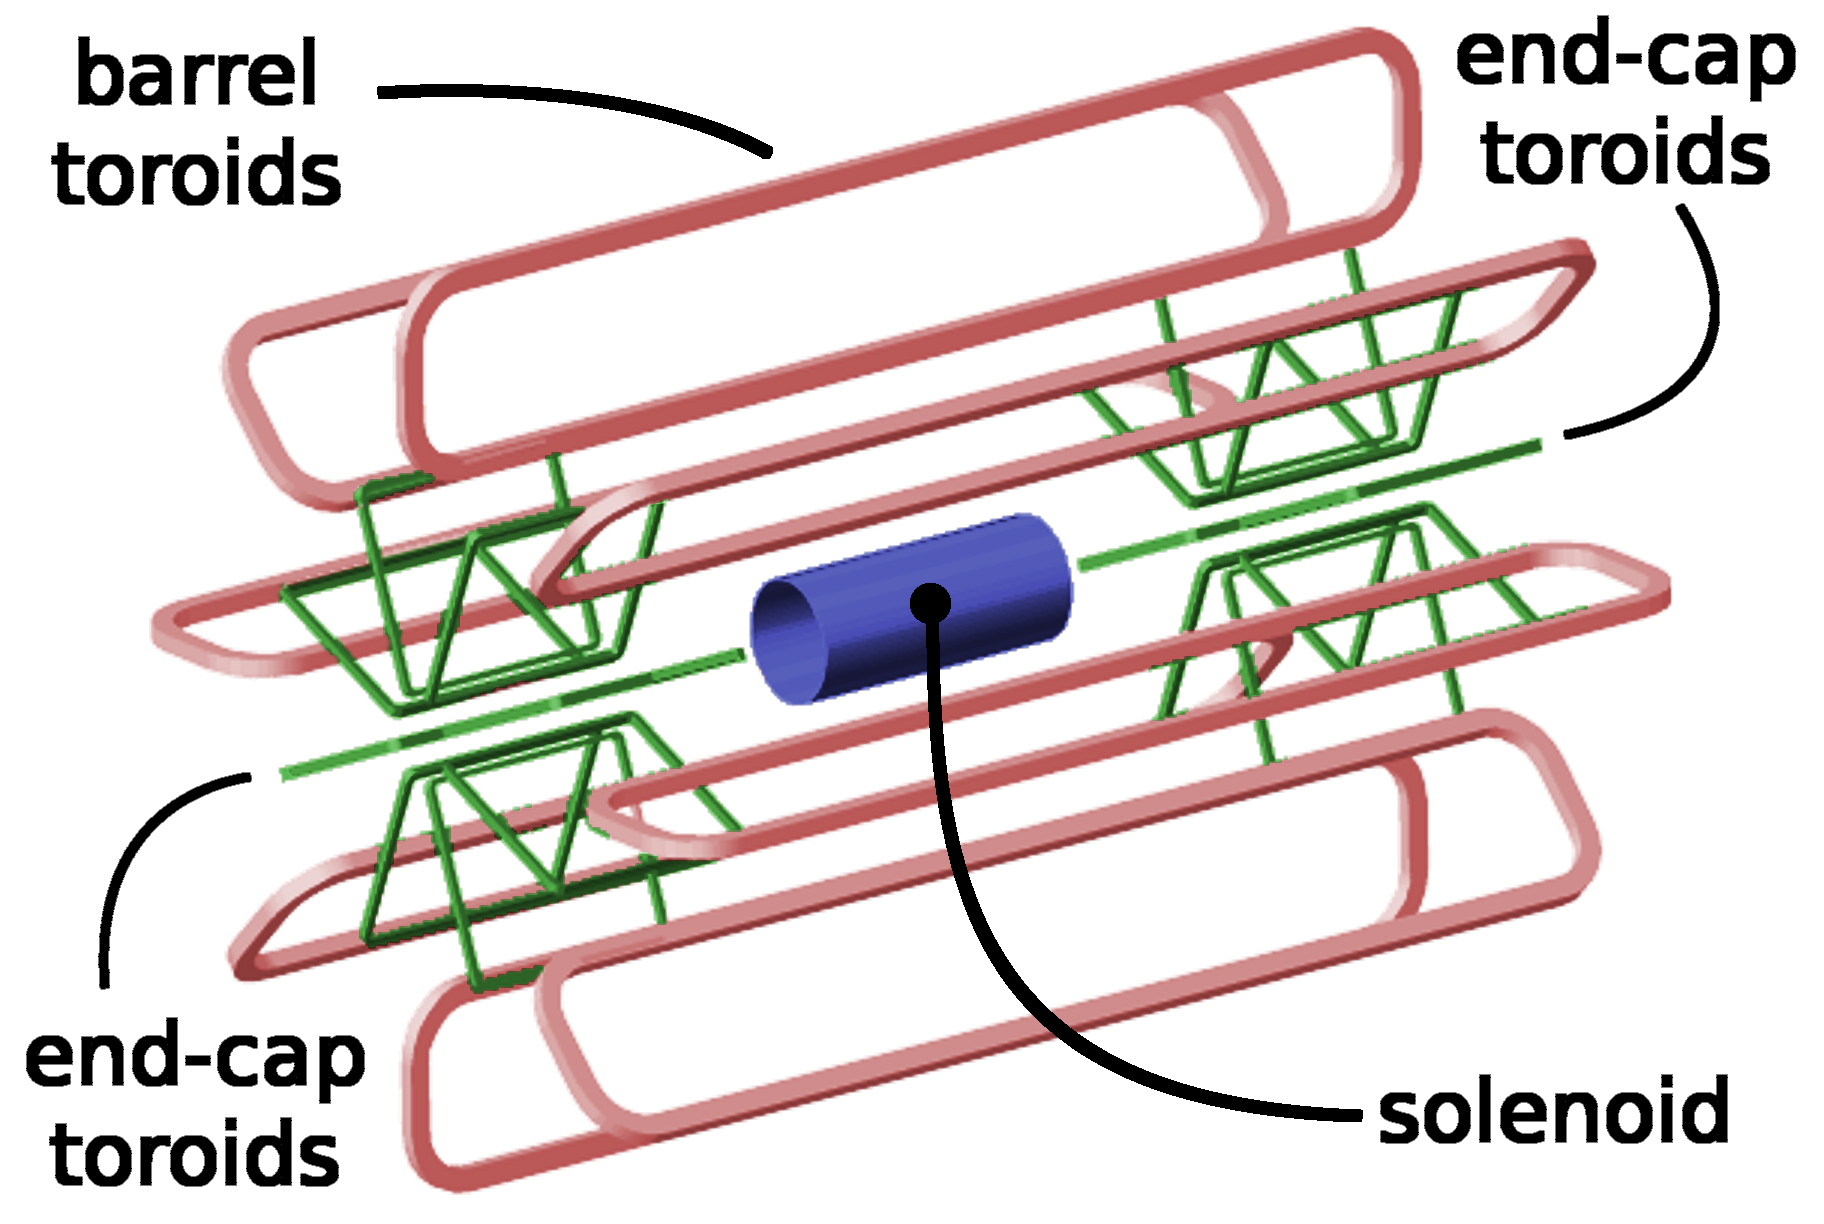
\includegraphics[width=\textwidth]{magnetSystems}
	\caption{ATLAS magnet system\cite{magnet_system_picture}.}
	\label{fig:magnet_system_picture}
\end{figure}

The current magnet system (Fig.\ref{fig:magnet_system_picture}) comprises four superconducting magnets\cite{magnet_system}, for charged particles bending and momentum measurement in the $8000\ m^3$ volume of the apparatus.\\

The \textit{Central Solenoid Magnet} encloses the tracking volume and provides a $2\ T$ magnetic field and minimal thickness in order to reduce the degradation of photon and electron energy resolution in the subsequent calorimeter layers.\\

The \textit{Barrel} and \textit{Endcap Toroids} provide a tangential magnetic field of about $1\ T$ for the muon detectors, both in the radial and the forward region.\\

As the current magnet system already fulfils HL-LHC requirements, it will not require an
upgrade. [ref? NON SE NE PARLA NEL LOI/SCOPING]

\subsection{The Inner Detector}

\begin{figure} [h]
	\includegraphics[width=\textwidth]{IDLayout}
	\caption{ATLAS Inner Detector layout\cite{Aad:2008zzm}. IBL is not shown in this layout.}
	\label{fig:IDLayout}
\end{figure}

The ATLAS \textbf{Inner Detector} (ID), whose layout is shown if Fig.\ref{fig:IDLayout}, is designed to measure the momentum of the
charged particles tracks with $p_{T}$ larger than a typical threshold of $500\ MeV$ and 
within $|\eta| < 2.5$, identifying both primary and secondary vertices\cite{Aad:2008zzm}. \\

The ID is contained in a cylindrical envelope (with the axis along the z-axis) that extends
$\pm\ 3512\ mm$ in length and $1150\ mm$ in radius. The whole system is placed inside
a solenoid magnet which produces a field parallel to the beam line of $2\ T$(see sec.\ref{sec:magnet}). The ID is composed by three sub-detectors: the innermost section provides
high resolution pattern recognition using \textit{silicon pixel layers}, the middle one consists of stereo pairs of \textit{silicon microstrip} (SCT) layers and the outermost one consists of the \textit{Transition Radiation Tracker} (TRT). During 2014 ATLAS upgrade, the \textit{Insertable B-Layer} (IBL), a fourth pixel barrel layer, was added to avoid the decrease of performances after the luminosity upgrade. \\

Each one of these detectors is subdivided into a \textit{barrel} region, in which the sensor modules 
are organized tangentially with respect to a circle around the beam axis and an \textit{end-cap} region, in which they are placed perpendicularly with respect to the beam axis, producing
a disk resemblant shape.\\

The \textit{pixel} barrel layout consists of 3 layers placed at approximate radii $50.5\ mm$, $88.5\ mm$ and $122.5\ mm$ with respect to the beam 
axis. A fourth layer called \textit{Insertable B-Layer} (IBL) was added during the LS1 as the
innermost pixel layer at radius $32.7\ mm$. In the end-cap region, three disks per side were chosen,
at z position respectively $495\ mm$, $580\ mm$, $650\ mm$. \\

The \textit{SCT} barrel layout consists of four layers at radii $300\ mm$, $373\ mm$, $447\ mm$ and $520\ mm$. The end-cap region is instead composed by 9 disks per side with variable
inner radii and z-position ranging from $850\ mm$ to $2720\ mm$. \\

The \textit{TRT} barrel layout is formed by straws parallel to the beam axis (GIUSTO?) at radii from $563\ mm$ to $1066\ mm$,
while the end-cap region consists of radially wound straws with z ranging from $850\ mm$ to 
$2710\ mm$. 

\subsubsection*{Pixel and SCT} (DIFFERENZE CON TDR: dimensioni diverse dei singoli pixel)

The pixel and SCT sensors are designed to maintain their performance during the detector
lifetime at nominal luminosity\cite{Aad:2008zzm}. As the integrated radiation dose has significant consequences
on these sensors, they are operated at a temperature between $-10\ ^{\circ}C$ and $-5\ ^{\circ}C$.\\

\textit{Pixel sensors} of the Run 1 ID (thus excluding IBL) are $250\ \mu m$ thick detectors which are mounted on oxygenated n-type wafers, with the pixel on the $n^+$ side(??). About 90\% of the pixel on a sensor have a nominal 
size of $50 \times 400\ \mu m^2$, while the rest are $50 \times 600\ \mu m^2$ large and are placed
at the front-end chips on a module. There are a total of 1744 identical pixel sensors(modules??) with an external dimension of $19 \times 63\ mm^2$, each composed by 47232 pixels. For reasons of space, there are four ganged pixels on each column of the front-end chip, thus resulting in a total of 46080 readout channels. \\

\textit{IBL pixels} are, instead, $50 \times 250\ \mu m^2$ large to 
ensure a highly precise measurement of the coordinates near the interaction point\cite{IBL}. Two 
different technologies have been implemented in the central and forward IBL region, which
results in a different sensor thickness and chip size.\\

The \textit{SCT} consists of a total of 15912 sensors with thickness $285\ \pm\ 15\ \mu m$. Every sensor consists of 768 strips of $12\ cm$ length, with average pitch of $80\ \mu m$.
On each SCT module there are two back-to-back sensors with a relative angle of $40\ mrad$,
which allows the extraction of a second coordinate.

\subsubsection*{TRT}
The basic elements of \textit{TRT} consist of $4\ mm$ diameter tubes\cite{Aad:2008zzm}. For both the barrel
and end-cap sections, the anodes are made of $31\ \mu m$ diameter, $\pm\ 71.2\ cm$ 
active length tungsten wires 
connected to the front-end electronics and grounded. The wires are carefully aligned within
the straw, with a maximum tolerance of $300\ \mu m$. The barrel section contains about 
50000 straw tubes, whereas the end-cap contains approximatively 320000,
for a total of 420000 electronic channels\cite{ATLAS:1997ag}. This detector typically provides
an almost continuous tracking of the particles traversing it, with an average of 36 measurements per track.\\

\bigskip
The upgrade of the ID is the main focus of this thesis and will be covered in sec.\ref{sec:ITkLayouts}.


\subsection{Calorimeter system}

ATLAS experiment  relies on an electromagnetic and an hadronic calorimeter for the identification and the measurement of physical quantities of photons, electrons, hadrons and jets. 
Both compartments are divided into a central and a forward region (Fig.\ref{fig:current_Cals}).

\begin{figure} [h]
	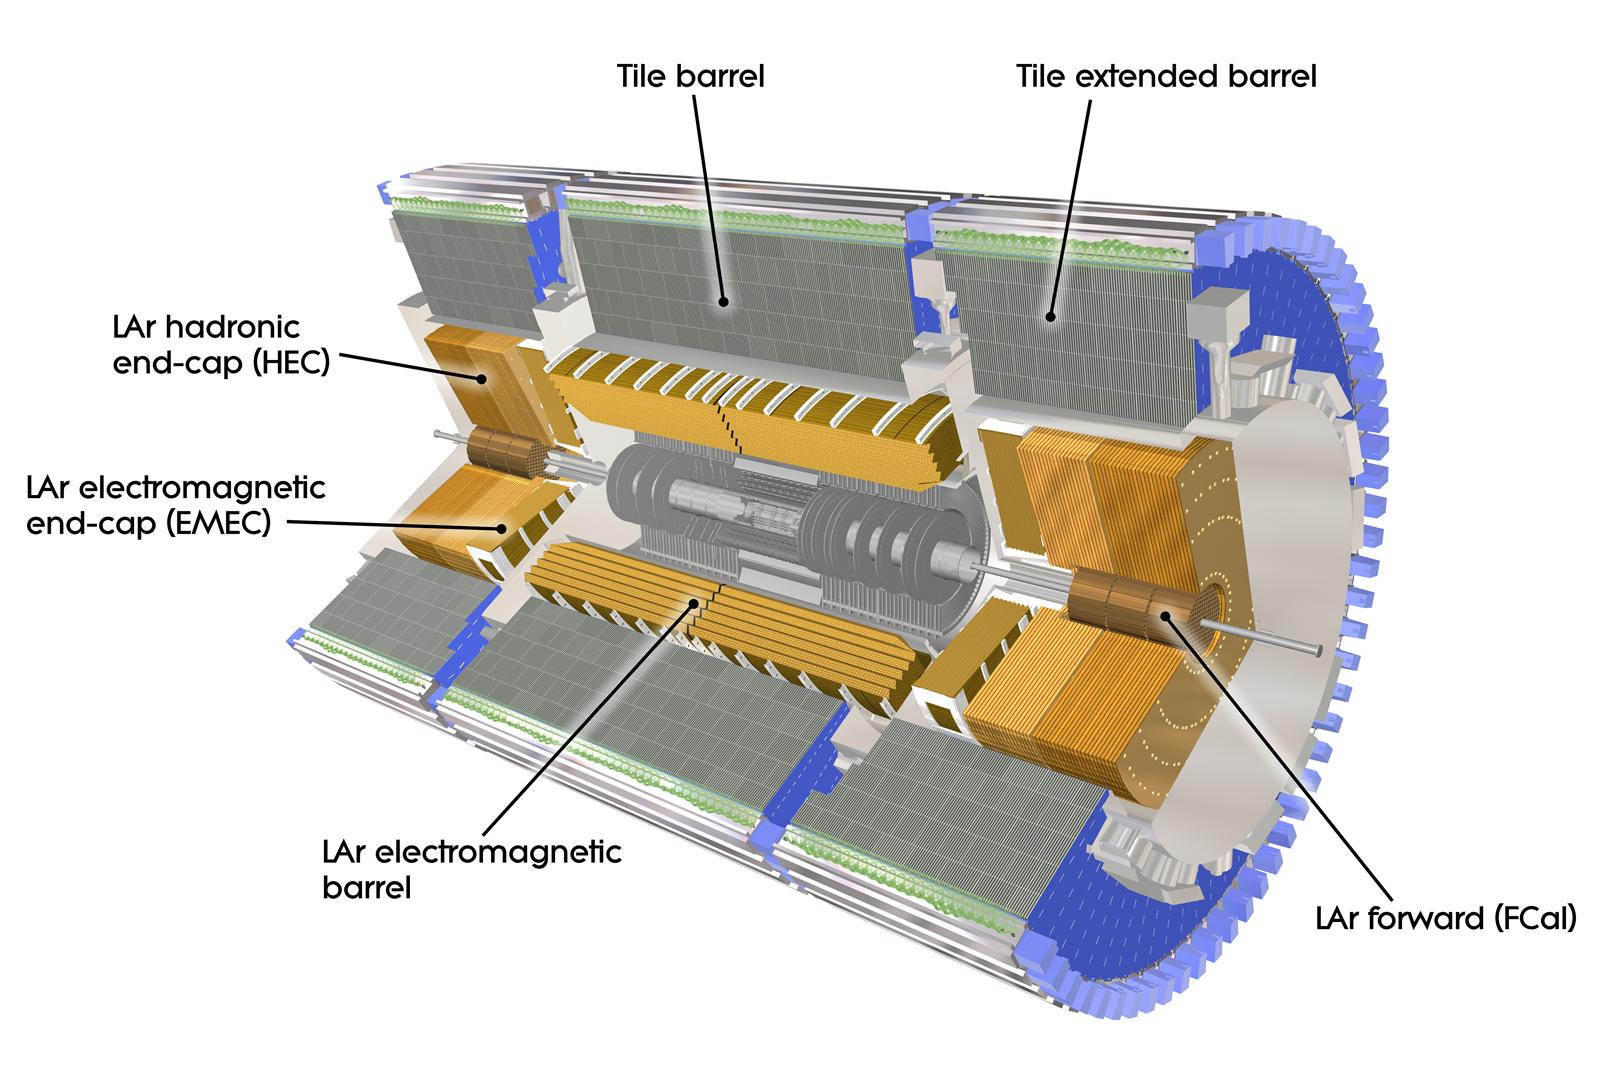
\includegraphics[width=\textwidth]{current_Cals}
	\caption{ATLAS Calorimeter System.}
	\label{fig:current_Cals}
\end{figure}

\subsubsection*{Liquid Argon Calorimeters}\label{sec:LAr}
Several components of the ATLAS calorimeter use liquid Argon (LAr) as active medium\cite{current_EMCal}. The electromagnetic barrel and endcap (EMEC) are entirely made up this way, but also the Hadronic Endcap Calorimeter (HEC) and the Forward Calorimeter (FCal). \\[2pt]
The \textbf{electromagnetic calorimeter} uses lead as absorber and is designed to trigger on and to provide precision measurements of electrons, photons, jets, and missing $E_T$ .
The full cryostat of the \textit{barrel section} is $6.8\ m$ long, with the inner and outer radius being respectively $1.15\ m$ and $2.25\ m$ and ranges in $|\eta|$ from 0 to 1.7.  The \textit{endcap section} consists of two concentric wheels, the larger one ranging in $|\eta|$ from 1.4 to 2.5, the smaller from 2.5 to 3.2. In addition, a \textit{presampler} layer has been inserted behind the cryostat wall to allow measurement correction due to losses in the upstream material. 
%The amount of inactive material due to the solenoid
%accounts for $0.63\ X_0$ and, as cited in Sec.\ref{sec:magnet}, has been optimized. 
Detailed simulations based on the response to high energy photons and electrons have
measured the thickness of the calorimeter to be about $24\ X_0$ in the barrel and $26\ X_0$ in the endcap. Each section is physically divided into towers which produce the signal and are so responsible
for the granularity of the calorimeter.
High granularity is especially required in the central regions, where it reaches the value of 
$\Delta\eta\ \times\ \Delta\phi\ =\ 0.025\ \times\ 0.025$, sometimes allowing to combine the information
coming from the inner detector to improve rejection power.
\begin{comment}
 In this region it is possible to combine the signal of the calorimeter with the information coming from the inner detector to improve the rejection power of $\pi_0$ against photons. Indeed, granularity is less and less relevant to the overall performance with increasing $|\eta|$. 
\end{comment}
Hermeticity is also a very important feature for the measurement of missing $E_T$ and has been maximized using a transition gap between the barrel and endcap cryostats of 95 mm. \\

\textbf{HEC}\cite{hec} is a sampling calorimeter with copper absorber plates and consists of two wheels of outer radius $2.03\ m$, made of 32 identical modules. It ranges in $|\eta|$ from 1.4 to 3.2 and every half of it shares the cryostat with the EMEC and FCal. \\[2pt]

\textbf{FCal} has to cope with a high level of radiation, which makes it a particularly challenging detector. 

\begin{comment}
To avoid an excessive neutron albedo in the central cavity the detector is actually recessed by 
$1.2\ m$ with respect to the frontal face of the electromagnetic calorimeter. FCal is a high density mixed copper-tungsten calorimeter and covers the range of $3.0\ < |\eta|\ <\ 4.9$. 
\end{comment}

 The high material density employed allows to reach the required $9.5\ \lambda$ in a reduced space and to minimize the endcap calorimeter pileup signal.  \\[2pt]

\subsubsection*{Hadron Tile calorimeters}
The main requirement for the \textbf{Tile Calorimeter} is to reconstruct the energy of the jets produced in the collisions and, due to the high center-of-mass energy at LHC, it has to assure 
high performances in a wide range of energies. Thanks to the use of an extended barrel, the HEC and the FCal (see Sec.\ref{sec:LAr}), it also provides a good $p_T^{miss}$ reconstruction.\\

The Tile calorimeter is a sampling calorimeter composed by alternated layers of scintillating tiles as active medium and steel as an absorber. The signal is carried out from each module using optical fibres, which can run through the layers thanks to the laminated structure of the calorimeter. It is segmented and provides a resolution of
$\Delta\eta \times \Delta\phi\ = 0.1 \times 0.1$.\\
The Tile Calorimeter is made up of one barrel ($5.64\ m$ long) and two extended barrel ($2.91\ m$ long) parts, with a gap of $60\ cm$ in between. It consists of a cylindrical structure of inner radius $2.28\ m$ and $4.23\ m$. The barrel covers the region $0\ <\ |\eta|\ <\ 1.0$ whereas the extended barrel covers the region $0.8\ <\ |\eta|\ <\ 1.7$. The overlap region from 0.8 to 1.0 is
occupied by the Intermediate Tile Calorimeter (ITC).\\

\subsubsection*{Upgrade of the electromagnetic calorimeter}

The performance required by HL-LHC barrel electromagnetic calorimeter is the same as the current one, thus it does not need to be upgraded. In contrast to that, the FCal performances will be degraded by the conditions of HL-LHC. In the Reference Scenario of the ATLAS Scoping Document\cite{scoping} the replacement of the current FCal with a high-granularity Small-Gap Forward Calorimeter (sFCal) is foreseen, which is superior to the current one in terms of resolution and size of LAr gaps. These latter are designed to be smaller than the current in order to reduce the risk of formation of Argon bubbles, due to the high energy release. (??) The improvement in granularity would be also required by the extension in $|\eta|$ of the Inner Detector in the aforementioned scenario (??). Also, the addition of a High Granularity Timing Detector (HGTD) is planned, which will be hopefully installed in front of the LAr Calorimeter endcaps and will be needed to reduce the (OUT-OF-TIME?) pileup signal. It will cover the range $2.4\ <\ |\eta|\ <\ 4.3$ and it will measure the arrival time of charged particles, assigning them to different collision vertices. The readout electronics will also need to be upgraded due to insufficient radiation tolerance and poor performance with respect to that necessary for the foreseen trigger upgrade. In the Middle and Low cost 
scenarios, on the contrary, no upgrades in the endcap and forward region are foreseen, unless the risk of formation of Argon bubbles is considered too high, in which case a MiniFCal will be installed in front of the existing FCal. \\

\subsubsection*{Upgrade of the Tile Calorimeter}

The Tile Calorimeter maintains the required performance even during the HL-LHC phase and
so it does not need replacement. On the contrary, the readout electronics will need to be upgraded due to limited radiation tolerance and to accommodate the new trigger requirements in terms of rates and latencies. This will be fulfilled, as in the case of the LAr (see
Sec.\ref{sec:LAr}), by substituting the on-detector front-end electronics, the optical links, the off-detector signal processing unit, the powering system and the interface modules to the TTC and DAQ systems. (??).

\subsection{Muon Spectrometer}\label{sec:muon}\cite{muon_tdr}\cite{Aad:2008zzm}

\begin{figure} [h]
	\centering
	\includegraphics[scale=0.4]{muonSystem}
	\caption{ATLAS Muon System\cite{muon_tdr}.}
	\label{fig:muonSystem}
\end{figure}

ATLAS \textbf{muon spectrometer} is designed to track charged particles that manage to pass through the whole calorimetric system and to perform stand-alone measurements of their momentum, in the range 
$3\ GeV < p_{T} < 3\ TeV$. Even at the upper limit, the detector is still able to provide adequate momentum resolution and charge sign measurement.\\

The layout of the current  ATLAS muon spectrometer is shown if Fig. \ref{fig:muonSystem}. It is divided into three main regions of pseudorapidity: in the range $0.0 < |\eta| < 1.0$ the bending power
is provided by a barrel magnet composed by eight coils; the range $1.4 < |\eta| < 2.7$ is, instead, covered by a pair of \textit{end-cap toroids} placed at the tips of the barrel toroid; the \textit{transition
region}, $1.0 < |\eta| < 1.4$, is covered by a combination of the two. The system is built so that it provides a field that is mostly orthogonal to the particle direction while minimizing the contribution to multiple scattering. A \textit{trigger system} is also available for $|\eta| < 2.4$. \\

In the barrel section the tracks are measured by stations arranged in three concentric cylinders (approximatively $5\ m$, $7.5\ m$ and $10\ m$ radius) while in the end-cap and
transition region other three stations are arranged in disks along the z-axis (approximatively at  $|z| = 7.4\ m$, $10.8\ m$, $14\ m$ and $21.5\ m$). An extra disk is added in the transition
region to increase acceptance. A gap in the region $|\eta| < 0.1$ is necessary to allow for services. The layout is designed so that a track coming from the interaction point can traverse only three of the aforementioned stations.\\

Four different detector technologies are employed in this detector to optimize momentum reconstruction and trigger efficiency in the 
different regions.  \textit{Monitored drift tube chambers}(MDT) are employed in the barrel and endcap regions (except in the innermost endcap layer, where the particle flux is maximum) to provide precise z coordinate measurement in the bending plane. In the innermost endcap layer, instead, \textit{Cathode Strip Chambers}(CSC) are used to provide $R-\phi$ and time measurements. \\

For the muon trigger system, \textit{Resistive Plate Chambers}(RPC) were selected for the barrel region, while \textit{Thin Gap Chambers}(TGC) were selected for transition and endcap regions. Other
than achieving the triggering functionality, they also provide the coordinate on the non-bending plane to the MDTs. 

\subsubsection{Upgrade}\cite{scoping}
During the HL-LHC upgrade, the huge increase in the average number of pileup events leads to a series of difficulties that must be overcome by a corresponding performance improvement.\\

In particular, the innermost endcap layer will be substituted by \textit{New Small Wheels}(NSW) that combines small strip TGCs and MicroMegas chambers, both for triggering and 
precision tracking. The MDTs, together with the New Small Wheels, should already be able to provide an adequate performance and will not be substituted. Its read-out electronics, instead, will not 
be able to cope with the high hit rate and the new ATLAS L0/L1 trigger scheme, so it will have to be subtituted. The same also applies for the RPCs and TGCs. In the case of RPCs, moreover,
the gas gain will be lowered to ensure safety in the expected high rate environment and protract its life. New RPCs with increased rate capabilities will be instead placed in the innermost barrel layer to maintain a
good trigger efficiency, while new high resolution TGCs will substitute the present ones in the middle endcap disk to keep fake rate at a minimum.\\

The possibility to extend the coverage to $|\eta| < 4$ to identify muons and tag inner detector tracks in that range will be made possible by inserting micro-pattern gaseous or silicon pixel
detectors in the region $2.7 < |\eta| < 4.0$.

\subsection{Trigger and DAQ system}

\begin{figure} [h]
	\centering
	\includegraphics[scale=0.4]{trigger}
	\caption{ATLAS Trigger and DAQ System\cite{Green:2010zza}.}
	\label{fig:trigger}
\end{figure}

The current ATLAS \textbf{trigger system} is structured in three levels of event selection: \textit{Level 1} (L1), \textit{Level 2} (L2) and event filter\cite{Aad:2008zzm}. The L2 trigger, together
with the event filter, form the \textit{High-Level Trigger} (HLT). Due to the high level of integration between the HLT and the DAQ system they are sometimes referred as a single system (DAQ or 
DAQ-HLT)\cite{Green:2010zza}.\\

At LHC, a bunch crossing happens every 25 ns (i.e. $40\ MHz$), resulting in a trigger to the detector . The goal of L1 trigger is to search for signatures from high $p_{T}$ muons, electrons,
photons, jets and $\tau$ decaying into hadrons. It also searches for events with large $E_{T}^{miss}$ or large $E_{T}$. It manipulates reduced granularity data coming from the muon
spectrometer (RPCs and TGCs) and calorimeters. L1 trigger is designed to work with an accept rate of $100\ kHZ$, with a latency of $2.5\ \mu s$. A \textit{Central Trigger Processor} applies
the selection and, if the event passes it, the data is
sent to the DAQ and to the \textit{RoI Builder}, which computes the regions of interest for the next trigger level.
L2 trigger is designed to select events so that the event rate diminishes from the $100\ kHz$ of the L1 trigger to $3.5\ kHz$, with an average processing time of $40\ ms$ per event, by
exploiting a distributed architecture. This
level takes the regions of interest from the L1 trigger as input and send a data request to the network, based on these RoI. The events are distributed among the nodes and the selection is applied. If an event passes the selection it is sent to the \textit{event filter}, which applies a more sophisticated selection with high latency, taking the event rate from $3.5\ kHz$ to $\approx 200 Hz$, which are stored in a permanent memory area by the DAQ system.

\subsubsection{Upgrade}
The trigger system and electronics were designed to operate at the initial luminosity 
$\mathcal{L} = 10^{33} cm^{-2}s^{-1}$ at low trigger thresholds and at the Run2 upgrade
luminosity, $\mathcal{L} = 10^{34} cm^{-2}s^{-1}$, with higher thresholds\cite{scoping}.\\

With the increase of the luminosity to $\mathcal{L} = 2-3 \cdot 10^{34} cm^{-2}s^{-1}$ during
the Phase-I upgrade and then to a maximum of $\mathcal{L} = 7.5 \cdot 10^{34} cm^{-2}s^{-1}$, the entire TDAQ system will have to be significantly improved. During the Phase-I upgrade the NSW will be installed, together with a higher-granularity calorimeter
trigger and the L1 trigger will become more selective(?), keeping the latency and the accept rate unchanged. During this phase also the \textit{Fast TracKer trigger} (FTK)\cite{FTK_TDR} will be installed, which will perform
full tracking on the events accepted by the L1 trigger. \\

During the HL-LHC phase, when the luminosity will reach its maximum, it will be necessary
to increase the maximum rate and latency of the trigger system and install an additional Level 0 hardware trigger (L0), which relies on the muon and calorimeter trigger information. The L0 trigger is designed to decrease the data flow from $40\ MHz$ to $1\ MHz$, with a maximum latency of $6\ \mu s$. The upgraded L1 trigger will be seeded by the RoI provided by the L0
trigger and it will use full calorimeter readout with higher-granularity data. It is designed to
operate with a maximum latency of $30\ \mu s$ and an accept rate of $400\ kHz$ (in the Reference scenario\cite{scoping}). Finally, the Phase-II DAQ system is designed to make 
efficient use of commercial networking and computing hardware. 







\newpage
\section{Conclusions}\label{sec:conclusions}
\baselineskip 25pt
\baselineskip 5pt
\baselineskip 16pt

%%% EVENTUALE
\appendix

%%% OBBLIGATORIA:

\bibliographystyle{unsrt}
\bibliography{biblio}

\end{document}
